\documentclass[11pt,a4paper,titlepage]{article}
\usepackage[left=1.5cm,text={18cm, 25cm},top=2.5cm]{geometry}
\usepackage[utf8]{inputenc}
\usepackage{setspace}
\usepackage{graphicx}
\usepackage[czech]{babel}
\usepackage{float}
\usepackage{color}
\usepackage{hyperref}
\usepackage{fancyvrb}
\setlength{\parindent}{0cm}
\setlength{\parskip}{1em}
\sloppy

\hypersetup{
	colorlinks=true,
	linktoc=all,
	linkcolor=blue,
	citecolor=red,
	urlcolor=blue,
}

\begin{document}

		\setstretch{0.5}
		\begin{center}

			
\includegraphics[width = 150mm]{logo.png}\\

			\vspace{\stretch{0.382}}

			\LARGE
			Přenos dat, počítačové sítě a protokoly\\
			Hromadný projekt - Hybridní chatovací P2P síť\\
			\vspace{\stretch{0.618}}

		\end{center}

	\Large{\today} \hfill Jiří Matějka (xmatej52)
	\thispagestyle{empty}
	\newpage
	\setcounter{page}{1}

    \tableofcontents
	\newpage
	\newpage

    \section{Úvod} \label{uvod}
        Tato práce vznikla jako projekt do předmětu Přenos dat, počítačové sítě a protokoly na škole
		Vysoké učení technické v~Brně. Práce se zabývá implementace chatovací sítě nad transportním protokolem
        UDP. Síť se skládá z~libovolného počtu peerů a~minimálně jednoho registračního uzlu.

	\section{Struktura sítě} \label{struktura}
		Jak již bylo zmíněno v~úvodu, celá síť se skládá z~několika peerů a
        a~alespoň jednoho registračnního uzlu. K~registračním uzlům se připojují jednotliví peeři (uživatelé)
        a~právě od registračního uzlu získává každý uživatel informace o~dalších uživatelích v~síti.

        Uzel dále může navázat spojení s~jiným uzlem a navzájem si tak vyměnit záznamy
        o~registrovaných uživatelích a známých uzlech. Díky spojení mezi jednotlivými uzly
        může následně registrační uzel poskytnout informace i o~uživatelích, které nejsou
        registrovaní přímo u~něj, ale registrovali se k~některému z~jeho sousedů.

        \begin{figure}[htbp]
            \begin{center}
                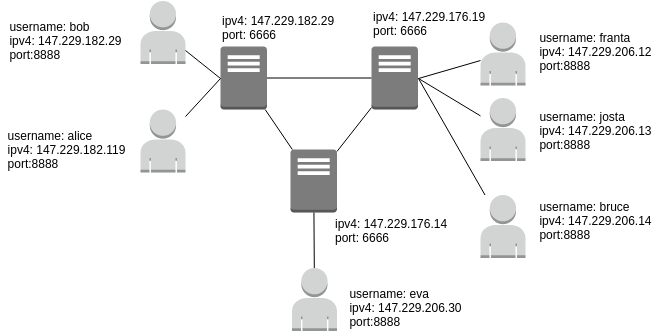
\includegraphics[scale=0.5]{base.png}
                \caption{Ukázka struktury sítě}
                \label{base}
            \end{center}
        \end{figure}

		\subsection{Peer}
            Každý uživatel v~síti je reprezentován peerem. Peer je v~síti identifikován unikátním uživatelským
            jménem, ipv4 adresou a portem. V~rámci operačního systému je identifikován pomocí unikátního ID.
            Každý uživatel je registrován k~právě jednomu registračnímu uzlu, který
            mu poskytuje informace o~ostatních uživatelých v~síti.

        \subsection{Uzel}
            Uzel je v~síti identifikován svou ipv4 adresou a portem. Každý z~uzlů si vede databázi známých uzlů a peerů. Uzel poskytuje informace
o~uživatelých v~síti pouze těm uživatelům, kteří jsou registrováni u~něj. Uzly si
            navzájem mezi sebou pravidelně vyměňují databáze peerů i uzlů. Pokud uzel obdrží informaci
            o~novém uzlu v~síti, naváže s~ním spojení.

    \section{Komunikace}
        Komunikace jednotlivých prvků v~síti je implementována pomocí jednoduchého komunikačního protokolu. Každá zpráva
        mezi dvěma prvky sítě je přenášena skrz UDP a před přenosem samotné zprávy je její obsah
        bencodován.

        \subsection{Komunikační prokol}
            V~rámci komunikačního protokolu bylo implementováno 8 různých zpráv. Každá z~těchto 8 zpráv má syntaxi
            JSON a všechny jejich atributy jsou povinné. Společnými atributy je potom typ zprávy, který identifikuje,
            o~jakou zprávu se jedná a txid, který nese unikátní identifikátor zprávy.

            \subsubsection{ACK}
                Zpráva \texttt{ACK} slouží k~potvrzení doručení zpráv typu \texttt{GETLIST}, \texttt{LIST}, \texttt{MESSAGE} a~\texttt{DISCONNECT}.
                V~komunikačním protokolu je implementována zejména proto, že UDP negarantuje doručení. Po odeslání výše uvedených zpráv
                se na zprávu \texttt{ACK} čeká maximálně po dobu 2 sekund, poté se předpokládá, že zpráva nebyla doručena.

                Zpráva má dva atributy -- txid a type, kde txid nese identifikátor zprávy, kterou zpráva \texttt{ACK} potvrzuje.
                Výsledná struktura zprávy tedy bude vypadat následovně: \verb+{"type":"ack", "txid":<ushort>}+

            \subsubsection{HELLO}
                Zpráva \texttt{HELLO} slouží k~registraci peeru k~uzlu. Pro udržení spojení mezi peerem a uzlem odesílá peer zprávu
                \texttt{HELLO} každých 10 sekund. Zpráva obsahuje kromě atributů type a txid další 3 atributy identifikující
                uživatele -- username, ipv4 a port. Pokud uzel neobdrží od uživatele po dobu 30 sekund žádnou zprávu \texttt{HELLO},
                uživatele odhlásí. Uživatele odhlásí i tehdy, pokud obdrží zprávu \texttt{HELLO} s~nulovou ipv4 adresou a portem.

                Struktara zprávy \texttt{HELLO} vypadá následovně:
\begin{verbatim}
{
    "type":"hello",
    "txid":<ushort>,
    "username":"<string>",
    "ipv4":"<dotted_decimal_IP>",
    "port":<ushort>
}
\end{verbatim}

            \subsubsection{UPDATE}
                \texttt{UPDATE} slouží k~navázání spojení mezi 2 uzly a výměny si informací o~registrovaných peerech a známých uzlech. Zpráva
                \texttt{UPDATE} tedy v~sobě nese seznam všech známých uzlů odesílatele včetně seznamu peerů, které jsou k~jednotlivým uzlům
                registrovány. Zpráva update se odesílá každé 2 sekundy a pokud uzel neobdrží od některého ze svých sousedů zprávu \texttt{UPDATE}
                po dobu 10 sekund, přeruší komunikaci s~tímto uzlem.

                Struktara zprávy \texttt{UPDATE} vypadá následovně:
\begin{verbatim}
{
    "type":"update",
    "txid":<ushort>,
    "db":{
        "<dotted_decimal_IP>,<ushort_port>":{
            "<ushort>":{
                "username":"<string>",
                "ipv4":"<dotted_decimal_IP>",
                "port":<ushort>
            }
        }
    }
}
\end{verbatim}

            \subsubsection{DISCONNECT}
                Po obdržení zprávy \texttt{DISCONNECT} přeruší uzel komunikaci s~odesílatelem (za předpokladu, že odesílatel je registrační uzel).
                \texttt{DISCONNECT} obsahuje pouze atributy typ a txid a její struktara vypadá následovně: \verb+{"type":"disconnect", "txid":<ushort>}+
            \subsubsection*{GETLIST}
                Příkazu \texttt{GETLIST} využívá peer k~aktualizaci svého seznamu známých uživatelů v~síti. Zpráva \texttt{GETLIST} obsahuje pouze
                atributy txid a type a její strukturlze popsat následovně: \verb+{"type":"getlist", "txid":<ushort>}+
            \subsubsection{LIST}
                Zpráva \texttt{LIST} je odpovědí uzlu na příkaz \texttt{GETLIST} od peera. Zpráva nese v~sobě seznam všech známých
                uživatelů v~síti bez ohledu na to, k~jakému uzlu jsou registrovaní.

                Zpráva \texttt{LIST} vypadá následovně:
\begin{verbatim}
{
    "type":"list",
    "txid":<ushort>,
    "peers":{
        "<ushort>":{
            "username":"<string>",
            "ipv4":"<dotted_decimal_IP>",
            "port":<ushort>
        }
    }
}
\end{verbatim}
            \subsubsection{MESSAGE}
                Zprávu \texttt{MESSAGE} použije peer, pokud chce zaslat zprávu jinému peeru. Posílání zpráv \texttt{MESSAGE}
                probíhá pouze mezi peery navzájem a registračních uzlů se tato zpráva vůbec netýká. \texttt{MESSAGE} kromě
                atributů txid a type nese ještě atribut identifikující odesílatele (from), příjemce (to) a atribut nesoucí obsah
                zprávy (message).
\begin{verbatim}
{
    "type":"message",
    "txid":<ushort>,
    "from":"<string>",
    "to":"<string>",
    "message":"<string>"
}
\end{verbatim}

            \subsubsection{ERROR}
                Tato zpráva se odesílá jako oznámení o~chybě (neobdržení zprávy \texttt{ACK}, špatný formát přijaté zprávy, neregistrovaný užiatel
                odeslal uzlu příkaz \texttt{GETLIST} apod.). Kromě atributů txid a type se ve zprávě nachází jště atribut verbose, jehož
                hodnota nese textový popis chyby. Zpráva \texttt{ERROR} vypadá tedy následovně: \verb+{"type":"error", "txid":<ushort>, "verbose":"<string>"}+

    \begin{figure}[htbp]
        \begin{center}
            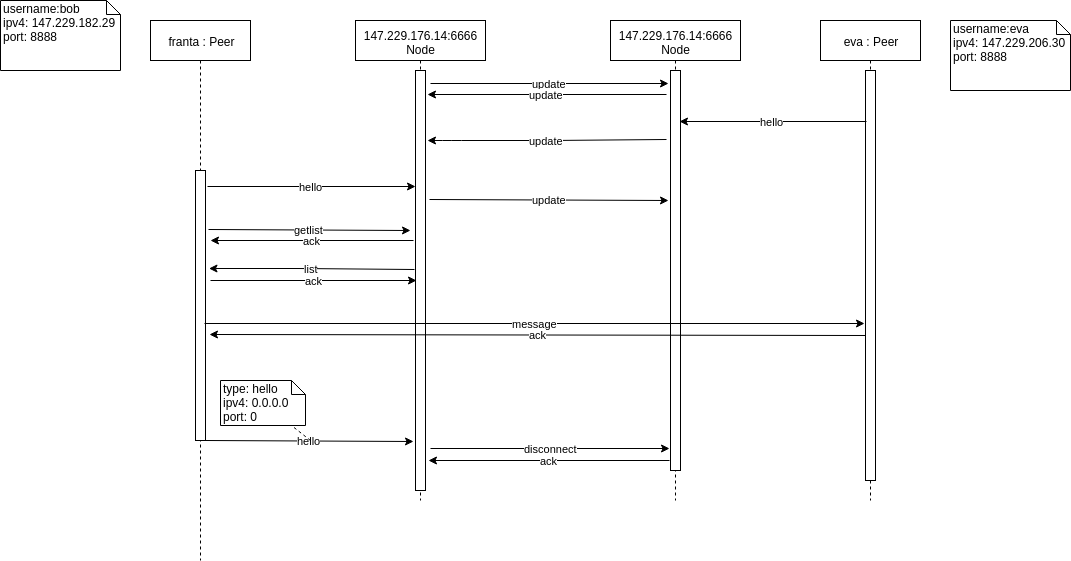
\includegraphics[scale=0.5]{protokol.png}
            \caption{Ukázka komunikace}
            \label{base}
        \end{center}
    \end{figure}

    \section{Implementace}
        Projekt je implementován v~jazyce python3 a samotná implementace je rozdělena do 7 modulů, které jsou společné pro uzly i peery.
        Veškerý příjem zpráv je implementován v~modulu \texttt{Receiver.py}, odesílání zpráv v~modulu \texttt{Sender.py}, registrace k~uzlu,
        navázání a udržení spojení uzly a udržení spojení mezi uzlem a peerm v~modulu \texttt{ConnectionKeeper.py}. Komunikační protokol je
        implementován v~modulu \texttt{Protokol.py}. Zbylé 3 moduly jsou \texttt{Functions.py},
        kde jsou obsaženy užitečné funkce používané napříč mezi moduly (např. zpracování argumentů), \texttt{FileLock.py} sloužící k~výlučnému přístupu
        k~souborům a \texttt{InputReader.py} který načítá příkazy ze souborů a standartního vstupu.

        \subsection{Registrační uzel}
            Aplikace registračního uzlu je implementována v~souboru \texttt{pds18-node.py}. Aplikaci lze ovládat zadáním příkazů na
            standartní vstup nebp pomocí aplikace RPC, která je popsána níže. Spuštění aplikace:


            \fontsize{11pt}{12pt}\verb+pds18-node.py --id N --reg-ipv4 IPV4 --reg-port PORT+
            \begin{itemize}
                \item \verb+--id+ -- Unikátní identifikátor uzlu v~rámci operačního systému
                \item \verb+--reg-ipv4+ -- IP adresa uzlu, na kterém bude uzel přijímat zprávy
                \item \verb+--reg-port+ -- Port uzlu, na kterém bude uzel přijímat zprávy
            \end{itemize}

            Po spuštění aplikace uzel vytvoří vlákno, které pravidelně kontroluje databázi známých sousedů a případně odesílá
            zprávy typu \texttt{UPDATE}. Dále vytvoří vlákno, které pravidelně kontroluje databázi registrovaných peerů a
            známých uzlů a případně tuto databázi promazává. Další vytvořené vlákno zpracovává přijaté zprávy a tvoří na ně
            odpovědi. V~neposlední řadě se vytvoří další vlákno, zpracovávající databázi očekávaných \texttt{ACK} zpráv.
            A~poslední 2 vlákna, co vzniknou, načítají příkazy ze souboru (kam je zadává aplikace RPC) a ze standartního
            vstupu (kam je zadává sám uživatel). Rodičovský proces pouze tyto příkazy předává ostatním vláknům a případně vypisuje
            chyby nebo zpracované informace na chybový nebo standartní výstup. Uzel tedy vytvoří dohromady 6 vláken.

            Během registrace peeru k~uzlu nebo synchronizaci 2 uzlů mohou nastat kolize mezi identifikátory jednotlových
            uživatelů. Pokud uzel detekuje kolizi během registrace peeru, odešle chybovou zprávu uživateli a registraci
            odmítne. Při kolizi během synchronizace databáze 2 uzlů odmítne pouze synchronizovat záznam uživatele, který
            způsobuje kolizi. V~tomto případě vygeneruje zprávu na chybový výstup a odešle chybovou zprávu druhému uzlu.
            Synchronizace ostatních peerů proběhne normálním způsobem.

            Podporované příkazy zadané na standartní vstup:
            \begin{itemize}
                \item \verb+\c ipv4 port+ -- Naváže spojení se zadaným uzlem
                \item \verb+\s+ -- Vynutí synchronizaci s~ostatnímy uzly
                \item \verb+\l+ -- Vypíše aktualní databázi uzlů a jejich peerů
                \item \verb+\n+ -- Vypise databázi znamých uzlů
                \item \verb+\d+ -- Odpojí se od ostatnich uzlů
                \item \verb+\h+ -- Vypíše nápovědu
                \item \verb+\exit+ -- Ukončí aplikaci
            \end{itemize}

        \subsection{Peer}
            Implementace apliakce peeru se nachází v~souboru \texttt{pds18-peer.py}. Stejně jako uzel, i~tuto aplikaci lze
            ovládat pomocí RPC nebo zadávání příkazů na standartní vstup. Spuštění aplikace:

            \verb+./pds18-peer.py --id N --reg-ipv4 IPV4 --reg-port PORT+

            \verb+                --chat-ipv4 IPV4 --chat-port PORT --username USERNAME+
            \begin{itemize}
                \item \verb+--id+ -- Unikátní identifikátor peeru v~rámci operačního systému
                \item \verb+--reg-ipv4+ -- IP adresa uzlu, ke kterému se peer zaregistruje
                \item \verb+--reg-port+ -- Port uzlu, ke kterému se peer zaregistruje
                \item \verb+--chat-ipv4+ -- IP adresa peeru, na které bude přijímat zprávy
                \item \verb+--chat-port+ -- Port peeru, na kterém bude přijímat zprávy
                \item \verb+--username+ -- Unikátní uživatelské jméno v~rámci celé sítě
            \end{itemize}

            Po spuštění aplikace se vytvoří vlákno, které provede registraci peeru k~uzlu a udržuje spojení
            pravidelným odesíláním zpráv typu \texttt{HELLO}. Dále se vytvoří vlákno, které zpracovává přijaté
            zprávy a vlákno, které zpracovává databázi očekávaných \texttt{ACK} zpráv. Protože ovlání aplikace je velmi
            podobné uzlu a je implementováno v~jednom modulu, i zde je zapotřebí dalších 2 vláken, která zpracovávající
            příkazy od uživatele a~RPC. Dohromady je pro jeden peer potřeba 5 vláken.

            Podporované příkazy zadané na standartní vstup:
            \begin{itemize}
                \item \verb+\l+ -- Vypíše seznam známých uživatelů
                \item \verb+\u+ -- Aktualizuje seznam uživatelů
                \item \verb+\r ipv4 port+ -- Připojí se na zadaný uzel
                \item \verb+\w username message+ -- Odešle zprávu zadanému uživateli
                \item \verb+\h+ -- Vypíše nápovědu
                \item \verb+\exit+ -- Ukončí aplikaci
            \end{itemize}
        \subsection{RPC}
            RPC slouží k~ovládání uzlu nebo peeru, pokud není možnost zadat příkazy na standartní vstup (například když proces uzlu běží na pozadí).
            Implementace RPC je umístěna v~souboru \texttt{pds18-rpc.py} a soubor lze spustit pomocí příkazu:

            \verb+./pds18-rpc --id N --peer|node --command CMD --PARAMETR_1 HODNOTA_1 --PARAMETR_2 HODNOTA_2 ...+
            \begin{itemize}
                \item \verb+--id+ -- Identifikátor peeru nebo uzlu, kterému bude předán příkaz
                \item \verb+--peer+ -- Určuje, že se jedná o~příkaz pro peer
                \item \verb+--node+ -- Určuje, že se jedná o~příkaz pro uzel
                \item \verb+--command+ -- Identifikátor příkazu
                \item \verb+--PARAMETR_1+ -- Parametr příkazu a jeho hodnota
            \end{itemize}

            Chování RPC je jednoduché. RPC po spuštění zpracuje zadané argumenty a zapíše příkaz do souboru. Peer nebo uzel
            následně soubor otevře a načte příkazy a vykoná je. Veškeré výpisy provádí peer nebo uzel, RPC pouze zadává
            příkazy do souboru.

            Na peeru jsou momentálně podporovány
            příkazy \texttt{message} (odeslání zprávy), \texttt{getlist} (aktualizace databáze známých uživatelů),
            \texttt{peers} (vypíše seznam peerů) a \texttt{reconnect} (změna registračního uzlu).
            Tyto příkazy se potom zadají při spuštění RPC následujícím způsobem:
            \begin{itemize}
                \item \verb+-command message --from USERNAME --to USERNAME --message TEXT+
                \item \verb+--command getlist+
                \item \verb+--command peers+
                \item \verb+--command reconnect --reg-ipv4 IPV4 --reg-port PORT+
            \end{itemize}

            Co se uzlu týče, jsou implementovány příkazy \texttt{database} (Zobrazí aktualní databázi peerů),
            \texttt{neighbors} (zobrazí aktuální databázy známých uzlů), \texttt{connect} (naváže komunikaci se zadaným uzlem),
            \texttt{disconnect} (přeruší komunikaci se všemy uzly) a \texttt{sync} (vynutí synchronizaci databází s~ostatnímy uzly).
            \begin{itemize}
                \item \verb+--command database+
                \item \verb+--command neighbors+
                \item \verb+--command connect --reg-ipv4 IPV4 --reg-port PORT+
                \item \verb+--command disconnect+
                \item \verb+--command sync+
            \end{itemize}

    \section{Testování}
        Testování projektu bylo provedeno ve spolupráci s~Lucií Pelantovou (implementace v~jazyce python), Janem Žárským (imlementace v~jazyce python),
        Martinou Zembjakovou (implementace v~jazyce python), Pavlem Dohnalíkem (implementace v jazyce Java) a Václavem Martinkou (implementace v~jazyce C\texttt{++}).
        Testování ukázalo, že mé řešení projektu je kompatibilní s~řešeným mých spolužáků. Během testováni byla odhalena v~mé implementaci jen 1 chyba,
        která se projevovala při odhlášení uživatele z~uzlu. Testování také prokázalo použitelnost implementovaných nástrojů nezávisle na RPC.
    \section{Závěr}
        Pomocí nástrojů vyvynutých v~rámci tohoto projektu lze sestavit chatovací síť stávající se z~uzlů a peerů. Implementace komunikačního
        protokolu je bez problému kompatibilní od implementace ostatních autorů. Díky načítání příkazů ze standartního vstupu lze uzel i peer
        jednoduše ovládat nezávisle na RPC. Díky RPC lze řídit jednoduše činnosti uzlů a peerů i jiným procesem a není problém je ovládat,
        když jsou spuštěny napozadí.

\end{document}
